\documentclass{article} % For LaTeX2e
\usepackage[table]{xcolor}
\usepackage{nips15submit_e,times}
\usepackage{hyperref}
\usepackage{verbatim}\usepackage{url}
\usepackage{natbib}
\usepackage[labelformat=simple]{subcaption}
\renewcommand\thesubfigure{(\alph{subfigure})}
\usepackage{multirow}
\usepackage{pgfplots, graphicx, amsmath,amsthm,amssymb,mathtools,   natbib,tikz}
\usetikzlibrary{arrows.meta, shadows, arrows, positioning}
%\usepackage{color}

\definecolor{SFUred} {RGB}{131,33,37}

\title{A Neural Network Approach to Classifying Banana Ripeness}

\author{
Kyle Demeule\\
Department of Computing Science\\
Faculty of Applied Sciences\\
Simon Fraser University\\
8888 University Drive\\
\texttt{kdd2@sfu.ca} \\
\And
Bernard S Chan \\
Department of Computing Science\\
Faculty of Applied Sciences\\
Simon Fraser University\\
8888 University Drive\\
\texttt{bernardc@sfu.ca} \\
\AND
Saeed Soltani\\
Department of Computing Science\\Faculty of Applied Sciences\\
Simon Fraser University\\
8888 University Drive\\
\texttt{saeeds@sfu.ca} \\
}

% The \author macro works with any number of authors. There are two commands
% used to separate the names and addresses of multiple authors: \And and \AND.
%
% Using \And between authors leaves it to \LaTeX{} to determine where to break
% the lines. Using \AND forces a linebreak at that point. So, if \LaTeX{}
% puts 3 of 4 authors names on the first line, and the last on the second
% line, try using \AND instead of \And before the third author name.

\newcommand{\fix}{\marginpar{FIX}}
\newcommand{\new}{\marginpar{NEW}}

\nipsfinalcopy % Uncomment for camera-ready version

\begin{document}


\maketitle

\begin{abstract}
In this paper, a new technique to detect the banana and its ripeness is introduced. This paper includes the methods and experiments that were implemented in the project. Some of the techniques that were used in this project includes classifying images by support vector machines in linear, radial basis functions and sigmoid functions. Also, we explain the optimization methods that used to improve the accuracy and decrease the number of features.\end{abstract}

\section{Introduction}

Traditionally, humans detect ripeness of fruit  through sight, odour, taste and touch. While people and animals are naturally equipped with these senses, machines are not, so automating fruit ripeness detection is a difficult task. Given that odor sensors and image processing are more reliable and developed than taste and touch, machine learning research in detecting fruit ripeness have been based around odor and and sight.  Through different type of odour sensors,~\citet{llobet1999non} and~\citet{li2007neural} collected smell information on ripening bananas and apples. Then, they applied various supervised classifier to classify their states.

Instead of odour, we are interested in integrating imaging and deep learning techniques to classify the ripeness of bananas. Based on reviews by~\citet{dadwal2012color} and~\citet{kodagali2012computer}, typical computer vision based ripeness detection methods are based on histogram matching or image segmentation. For example,~\citet{paulraj2009color} proposed a histogram-based neural network classifier for evaluating ripeness banana. Each image in the data set is decomposed into its RGB component and the number of pixels in each channel of varying intensities were counted. This information is then vectorized and fed into an neural network to be classified as unripe, ripe, or overripe. Segmentation based methods build on top of histogram-based methods. As mentioned in~\citet{dadwal2012color}, images are preprocessed so that the fruits in the picture are separated from the rest of the image. Then, classifying techniques, such as histogram-based neural network or clustering, are applied to classifying the ripeness. Segmentation based techniques are theoretically superior because features used for classification are only extracted from the relevant segmented region. 

With the works we have reviewed, the models only classify ripeness of fruits. In application, it is likely that there are other objects aside from the fruits on interest. Therefore, our first goal for this project is to implement a new method that could detect the ripeness of bananas. Secondly, our model will differentiate between banana and non-banana objects. Because the data sets from~\citet{paulraj2009color} is not available, our initial task is to create an appropriate data set. Then, instead of using histogram or segmentation based methods, we will use convolutional neural network (CNN) to extract features. With the features of each image at hand, we construct support vector machine (SVM) classification model to classify ripeness and whether the object in question is a banana. 

The remainder of this paper is organized as follows. In Section~\ref{sec:method}, we detail the steps in data generation, features extraction and label classification. The results from our experiment are discussed in Section~\ref{sec:results} and we conclude the paper with a discussion on our results and future work in Section~\ref{sec:conclusion}. 

\begin{comment}
\section {Background}
\begin{itemize}
\item literature review on fruit ripeness
\item literature review on neural network, deep learning, AlexNet
\item introduction to technologies used (Caffe, ScikitLearn)
\end{itemize}
\end{comment}
\section{Methodology}
\label{sec:method}
For this project, we created our own data set on banana and non-banana objects because the previous data sets from~\citet{saad2009recognizing} and~\citet{paulraj2009color} were not available. After establishing our own data set, we extracted the features of the images using a pre-trained convolution neural network. The Caffe deep learning frame work by~\citet{jia2014caffe} allowed us to access from many existing models. Given that we have a visualization task with different types of objects, we chose AlexNet by~\citet{krizhevsky2012imagenet} to extract the features. After obtaining the features of the images, we used the SVM library provided in SciKit Learn~\citep{scikit-learn} to classify the objects. A workflow of this project is shown as a flowchart in Figure~\ref{fig:flowchart}. In this section, we will discuss the details in each step of our work. 

\tikzstyle{block} = [rectangle, draw, fill=SFUred!20, 
    text width=30em, text centered, rounded corners, minimum height=2em]
    \tikzstyle{small} = [rectangle, draw, fill=white!20, 
    text width=5em, text centered, rounded corners, minimum height=2em]
        \tikzstyle{medium} = [rectangle, draw, fill=white!20, 
    text width=8em, text centered, rounded corners, minimum height=2em]

\tikzstyle{line} = [draw, -latex']

\begin{figure} [h]
\centering 
{
\begin{tikzpicture}[node distance = 1.2cm, auto,scale=.1]
    % Place nodes
    \node [block] (capture) {Capture images};
    \node [block, below of=capture] (process) {Label and process images (crop, resize and convert to RGB)};
%    \node [block, below of=process] (convert) {Convert to RGB };
    \node [block, below of= process] (cnn) {Extract features via CNN (Caffe and AlexNet)};
    \node [block, below of=cnn] (svm) {Classify data via SVM (SciKit Learn)};
    \node [medium, below left = 1cm and -10cm of svm] (nonbanana) {Non-Banana};
    \node [small, below right = 1.cm and -10 cm of svm] (banana) {Banana};
    \node [small, below of = banana] (ripe) {Ripe};
    \node [small, below left = . cm and .9 cm of banana] (unripe) {Unripe};
     \node [small, below right = .cm and .9 cm of banana] (overripe) {Overripe};

    % Draw edges
    \path [line] (capture) -- (process);
    \path [line] (process) -- (cnn);
%    \path [line] (convert)--(cnn);
    \path [line] (cnn)--(svm);
    \path [line] (svm)--(nonbanana);
        \path [line] (svm)--(banana);
          \path [line] (banana)--(unripe);
        \path [line] (banana)--(overripe);
	\path [line] (banana)--(ripe);
\end{tikzpicture}
}
\caption{A flow chart of project development.}
\label{fig:flowchart}
 \end{figure}


\subsection{Generating and Preparing the Data set}

Since the data sets used by~\citet{saad2009recognizing} and~\citet{paulraj2009color} were not publicly available, we decided to create on our own data set. Controlling for lighting, background and camera (Canon S90), we took pictures of banana and various non-banana objects. After the pictures were taken, we incorporated each picture at $0\,^{\circ}$, $90\,^{\circ}$, $180\,^{\circ}$ and  $270\,^{\circ}$ of rotation to increase the number of pictures in the data set by four fold. Also, there were equal number of pictures for each of the four labels: unripe banana, ripe banana, overripe banana and non-banana. For the banana data set, twelve unique bananas were used. We used apples, tomatoes, lemons, limes, mushrooms, broccolis, potatoes, pears and green peppers as non-banana objects. In total, there were 928 images generated for the data set and sample pictures of this data set are shown in Figure~\ref{fig:sampleDataset}. After obtaining the data set, we used various Python scripts to standardize the images so that each one is resized and cropped to $256\times 256$ pixels. Furthermore, each picture is decomposed into the RGB channels for features extraction. 

\begin{figure}[h]
\centering
 %%%%%% unripe %%%%%%%%%
  \begin{subfigure}{.123\textwidth}
  \centering
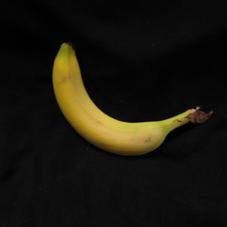
\includegraphics[width=\textwidth]{1_1.jpg}
\end{subfigure}%
 \begin{subfigure}{.123\textwidth}
  \centering
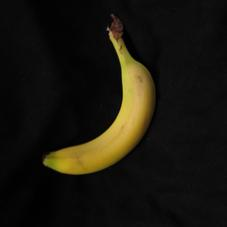
\includegraphics[width=\textwidth]{1_2.jpg}
\end{subfigure}%
  \begin{subfigure}{.123\textwidth}
  \centering
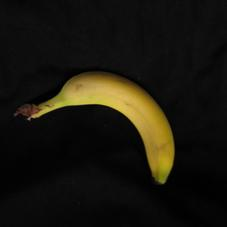
\includegraphics[width=\textwidth]{1_3.jpg}
\end{subfigure}%
  \begin{subfigure}{.123\textwidth}
  \centering
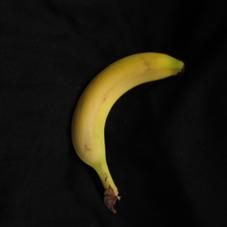
\includegraphics[width=\textwidth]{1_4.jpg}
\end{subfigure}\, %%%%%% ripe %%%%%%%%%
  \begin{subfigure}{.123\textwidth}
  \centering
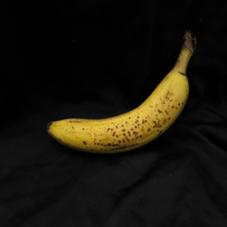
\includegraphics[width=\textwidth]{2_1.jpg}
\end{subfigure}%
 \begin{subfigure}{.123\textwidth}
  \centering
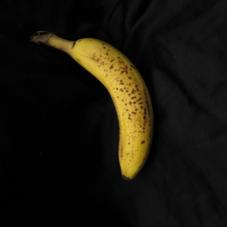
\includegraphics[width=\textwidth]{2_2.jpg}
\end{subfigure}%
  \begin{subfigure}{.123\textwidth}
  \centering
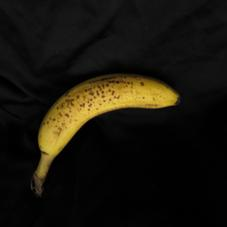
\includegraphics[width=\textwidth]{2_3.jpg}
\end{subfigure}%
  \begin{subfigure}{.123\textwidth}
  \centering
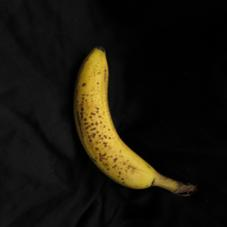
\includegraphics[width=\textwidth]{2_4.jpg}
\end{subfigure}%
\vskip .05in
 %%%%%% overripe %%%%%%%%%
  \begin{subfigure}{.123\textwidth}
  \centering
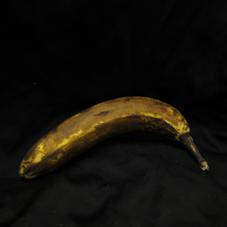
\includegraphics[width=\textwidth]{0_1.jpg}
\end{subfigure}%
 \begin{subfigure}{.123\textwidth}
  \centering
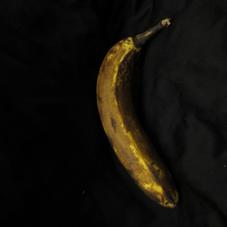
\includegraphics[width=\textwidth]{0_2.jpg}
\end{subfigure}%
  \begin{subfigure}{.123\textwidth}
  \centering
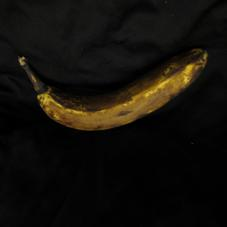
\includegraphics[width=\textwidth]{0_3.jpg}
\end{subfigure}%
  \begin{subfigure}{.123\textwidth}
  \centering
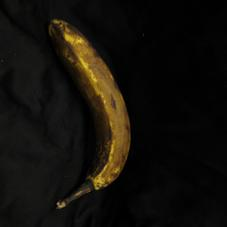
\includegraphics[width=\textwidth]{0_4.jpg}
\end{subfigure}\,
 %%%%%% non banana %%%%%%%%%
  \begin{subfigure}{.123\textwidth}
  \centering
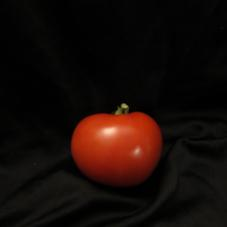
\includegraphics[width=\textwidth]{3_1.jpg}
\end{subfigure}%
 \begin{subfigure}{.123\textwidth}
  \centering
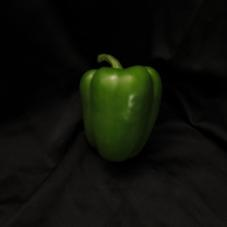
\includegraphics[width=\textwidth]{3_5.jpg}
\end{subfigure}%
  \begin{subfigure}{.123\textwidth}
  \centering
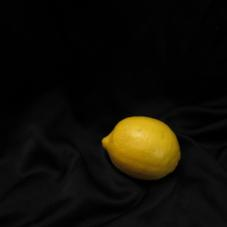
\includegraphics[width=\textwidth]{3_17.jpg}
\end{subfigure}%
  \begin{subfigure}{.123\textwidth}
  \centering
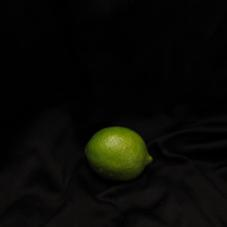
\includegraphics[width=\textwidth]{3_13.jpg}
\end{subfigure}%
\caption{Upper left: unripe bananas. Upper right: ripe bananas. Lower left: overripe bananas. Lower Right: non-banana objects.}
\label{fig:sampleDataset}
\end{figure}

 
\subsection{Features Extraction via AlexNet}

Features extraction is a challenging endeavor in image processing. Fortunately, there are a number of readily available algorithms for this purpose. Instead of building and training a model for features extraction from scratch, we installed Caffe, a deep learning framework developed by~\citet{jia2014caffe}, to assist us. We chose this platform because there exists many feature extraction models in the associated ``model zoo'' to choose from. 

From the many models availabe, we chose AlexNet developed by~\citet{krizhevsky2012imagenet} to extract features from our data set. Originally, this model was trained on 1.2 million high resolution images from the LSVRC-2010 training set. These images were initially labeled into 1000 different categories manually. As shown in Figure~\ref{fig:alexnet}, the CNN is a highly connected structure. This model consists of five convolutional layers and three fully connected layers and each layer could perform feature extraction and classification. Given its first place performance in ILSVRC-2012 in extracting features and classifying images, this model is an appropriate choice for our project.  

Using this pre-trained CNN, we extracted representation of the data set from the last three layers: FC6, FC7 and FC8. Internal representation of the first two layers are vectors of length 4096 and for FC8 is a vector of length1000.
\begin{figure}[h]
\centering
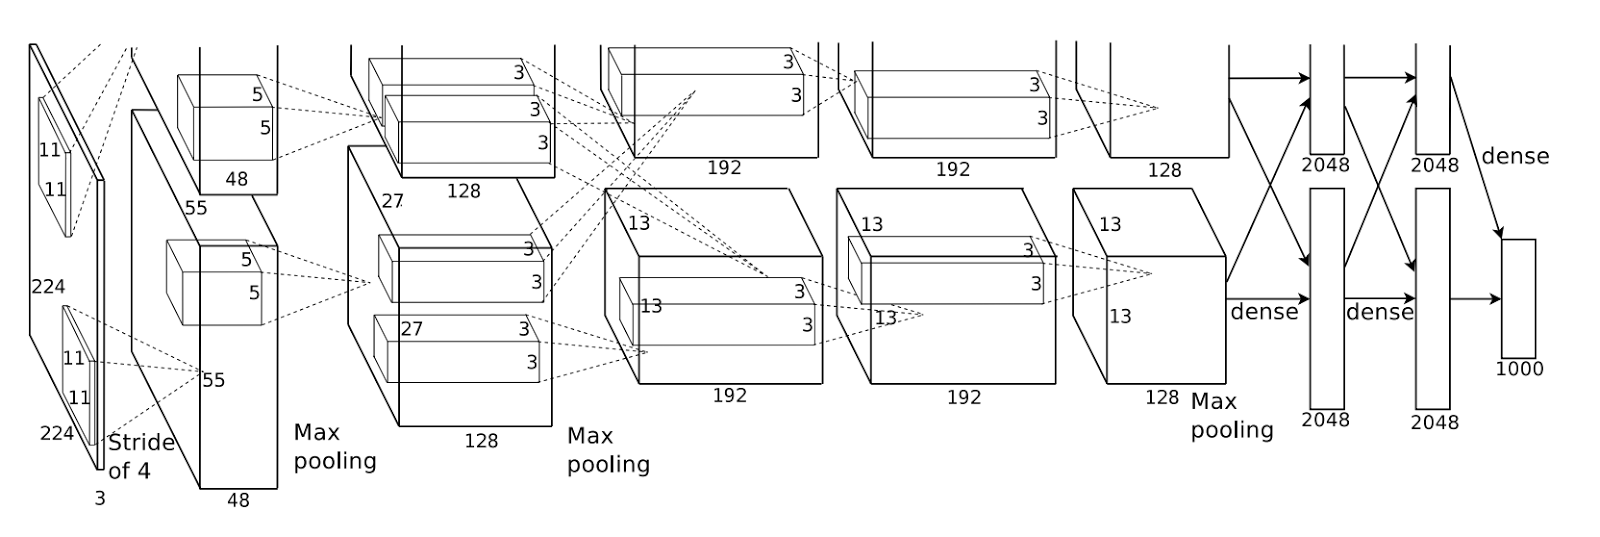
\includegraphics[width=\textwidth]{alexnet.png}
\caption{Architechture of AlexNet.}
\label{fig:alexnet}
\end{figure}

\subsection{Classification}
\label{sec:classification}
 \begin{itemize}
  \item Each set of four rotated pictures were either in the train or test set. 
  \item SciKit Learn~\citep{scikit-learn}: a Python library of machine learning algorithms. 
 \begin{itemize}
 \item Applied C-Support Vector Classification (\emph{sklenar.svm.svc}) to the extracted features for classification. 
 \item Linear, RBF, sigmoid and polynomial kernels were compared. 
 \item Parameters optimization through exhaustive grid search (\emph{sklearn.grid\_search}).
 \item optimized method based on training set
 \item cross-validation is built into the scikit learn grid search
 \item make sure people know that all the results come from one run. 
 \end{itemize}
 \end{itemize}
 
 \section{Results}
 \label{sec:results}
As mentioned in Section~\ref{sec:classification}, we applied existing SVM algorithms from SciKit Learn's library to classify the data in our set. For the experiment, we compared the performance of different kernels and feature extraction points from AlexNet. As highlighted in red in Table~\ref{tab:core}, using features extracted from RC6 and RC7 along with the radial basis function kernel both 
provided 100\% accuracy in training. Testing results were consistent with our training results and the \{FC6, RBF\} pair outperformed all other classifiers at 87.8\% accuracy. Therefore, the remainder of this report focuses on \{FC6, RBF\} as the chosen classifier. 

\begin{table}[h]
\caption{Overall accuracy of correctly classified objects from training and testing of SVM models with various kernels. Features were obtained from FC6, FC7 and FC8 exits of AlexNet. (Lin = linear, RBF = radial basis function, Sig = sigmoid, Poly = polynomial)}
\label{tab:core}
\centering
\begin{tabular}{|c|c|c|c|c|c|c|c|c|}\hline
 &  \multicolumn{4}{c|}{Training} & \multicolumn{4}{c|}{Testing}\\\hline
&Lin& RBF&Sig&Poly&Lin& RBF&Sig&Poly\\\hline
FC6&0.942&\cellcolor{SFUred!25}1.000&0.266&0.911&0.821&\cellcolor{SFUred!25}0.878&0.218&0.814\\\hline
FC7&0.876&\cellcolor{SFUred!25}1.000&0.266&0.872&0.788&0.862&0.218&0.804\\\hline
FC8&0.768&0.998&0.266&0.807&0.676&0.843&0.278&0.696\\\hline
\end{tabular}
\end{table}

To better understand the performance of the \{FC6, RBF\} classifier, we present the results on specific labels in Tables~\ref{tab:ripenessMatrix} and~\ref{tab:objectMatrix}. As seen in Table~\ref{tab:ripenessMatrix}, there was no confusion between unripe and overripe bananas. All errors in classifying banana centered around ripe bananas. As for the performance of classifying bananas versus other objects, Table~\ref{tab:objectMatrix} shows that there are more objects that are misidentified than bananas misidentified as other objects. 


	
\begin{table}[h]
\centering
\caption{Confusion matrix on banana ripeness with the \{FC6, RBF\} classifier. }
\label{tab:ripenessMatrix}
\begin{tabular}{|c|c|c|c|c|}\hline
&&\multicolumn{3}{c|}{Predicted}\\\hline
&&Unripe&Ripe&Overripe\\\hline
\multirow{3}{*}{Actual}&Unripe&\cellcolor{SFUred!65}0.913&\cellcolor{SFUred!15}0.095&0.000\\\cline{2-5}
&Ripe&\cellcolor{SFUred!15}0.068&\cellcolor{SFUred!65}0.836&\cellcolor{SFUred!15}0.096\\\cline{2-5}
&Overripe&0.000&\cellcolor{SFUred!15}0.033&\cellcolor{SFUred!65}0.967\\\hline
\end{tabular}
\end{table}

\begin{table}[h]
\centering
\caption{Confusion matrix on banana versus other objects with the \{FC6, RBF\} classifier. }
\label{tab:objectMatrix}
\begin{tabular}{|c|c|c|c|}\hline
&&\multicolumn{2}{c|}{Predicted}\\\hline
&&Banana&Other\\\hline
\multirow{2}{*}{Actual}&Banana&\cellcolor{SFUred!65}0.953&\cellcolor{SFUred!15}0.046\\\cline{2-4}
&Other&\cellcolor{SFUred!15}0.066&\cellcolor{SFUred!65}0.934\\\hline
\end{tabular}
\end{table}

To better understand the incorrectly classified objects from \{FC6, RBF\}, images of correctly and incorrectly classified objects are shown in Figure~\ref{fig:correctVsIncorrect}. Given the size of the data set, it is impractical to present the entire list of correctly or incorrectly identified objects for each class label in the figure. While we have only shown a selected few of the incorrectly classified objects, they are generally representative of the objects that were misclassified.

From the first two rows of Figure~\ref{fig:correctVsIncorrect}, we see that unripe and ripe bananas are often misclassified as each other. This observation correspond with the results shown in Table~\ref{tab:ripenessMatrix}. Furthermore, from the fourth row of Figure~\ref{fig:correctVsIncorrect}, we see that the objects that are misclassified as non-bananas are mostly overripe bananas. This information cannot be directly obtained from Table~\ref{tab:objectMatrix}.

\begin{figure}[h]
\centering
 %%%%%% unripe %%%%%%%%%
  \begin{subfigure}{.123\textwidth}
  \centering
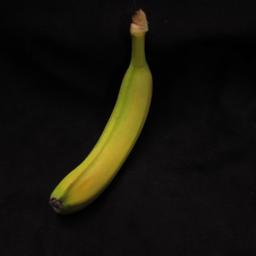
\includegraphics[width=\textwidth]{../results/q_samples/cor_pre.jpg}
\captionsetup{labelformat=empty}
\caption{Unripe}
\end{subfigure}%
\qquad
 \begin{subfigure}{.123\textwidth}
  \centering
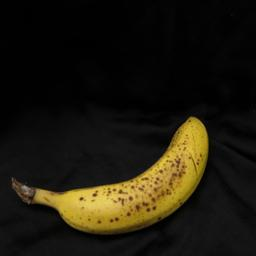
\includegraphics[width=\textwidth]{../results/q_samples/mis_pre/RIPE_1_PRE_1.jpg}
\captionsetup{labelformat=empty}
\caption{}
\end{subfigure}%
  \begin{subfigure}{.123\textwidth}
  \centering
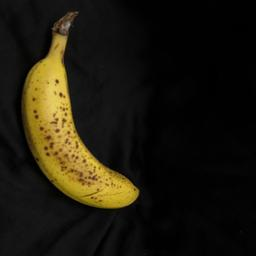
\includegraphics[width=\textwidth]{../results/q_samples/mis_pre/RIPE_1_PRE_3.jpg}
\captionsetup{labelformat=empty}
\caption{}
\end{subfigure}%
  \begin{subfigure}{.123\textwidth}
  \centering
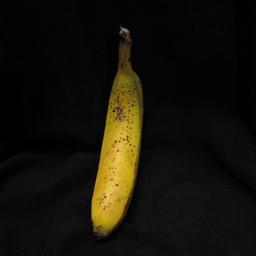
\includegraphics[width=\textwidth]{../results/q_samples/mis_pre/RIPE_1_PRE_4.jpg}
\captionsetup{labelformat=empty}
\caption{}
\end{subfigure}%
  \begin{subfigure}{.123\textwidth}
  \centering
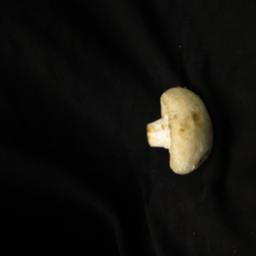
\includegraphics[width=\textwidth]{../results/q_samples/mis_pre/OTHER_1_PRERIPE_1.jpg}
\captionsetup{labelformat=empty}
\caption{}
\end{subfigure}
\vskip .1in
%%%%%% ripe %%%%%%%%%
 \begin{subfigure}{.123\textwidth}
  \centering
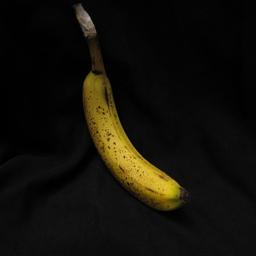
\includegraphics[width=\textwidth]{../results/q_samples/cor_ripe.jpg}
\captionsetup{labelformat=empty}
\caption{Ripe}
\end{subfigure}%
\qquad
 \begin{subfigure}{.123\textwidth}
  \centering
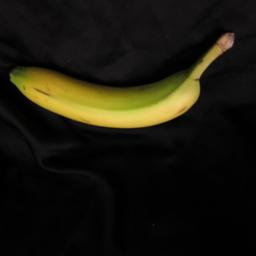
\includegraphics[width=\textwidth]{../results/q_samples/mis_ripe/PRE_2_RIPE_1.jpg}
\captionsetup{labelformat=empty}
\caption{}
\end{subfigure}%
  \begin{subfigure}{.123\textwidth}
  \centering
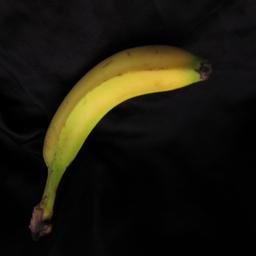
\includegraphics[width=\textwidth]{../results/q_samples/mis_ripe/PRE_2_RIPE_4.jpg}
\captionsetup{labelformat=empty}
\caption{}
\end{subfigure}%
  \begin{subfigure}{.123\textwidth}
  \centering
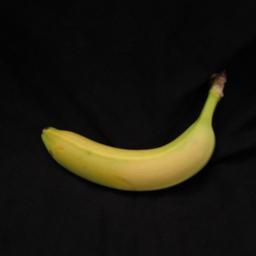
\includegraphics[width=\textwidth]{../results/q_samples/mis_ripe/PRE_2_RIPE_5.jpg}
\captionsetup{labelformat=empty}
\caption{}
\end{subfigure}%
  \begin{subfigure}{.123\textwidth}
  \centering
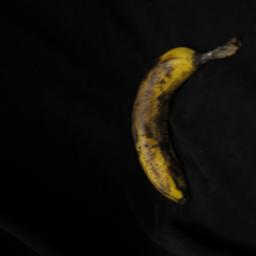
\includegraphics[width=\textwidth]{../results/q_samples/mis_ripe/ROTTEN_2_RIPE_2.jpg}
\captionsetup{labelformat=empty}
\caption{}
\end{subfigure}
\vskip .1in
 %%%%%% overripe %%%%%%%%%
  \begin{subfigure}{.123\textwidth}
  \centering
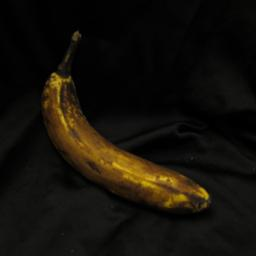
\includegraphics[width=\textwidth]{../results/q_samples/cor_rotten.jpg}
\captionsetup{labelformat=empty}
\caption{Overripe}
\end{subfigure}%
\qquad
 \begin{subfigure}{.123\textwidth}
  \centering
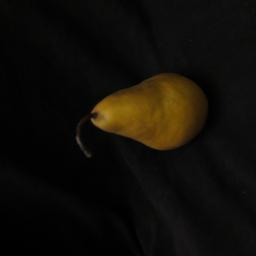
\includegraphics[width=\textwidth]{../results/q_samples/mis_rotten/OTHER_0_ROTTEN_1.jpg}
\captionsetup{labelformat=empty}
\caption{}
\end{subfigure}%
  \begin{subfigure}{.123\textwidth}
  \centering
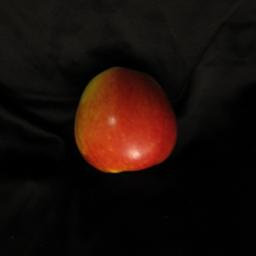
\includegraphics[width=\textwidth]{../results/q_samples/mis_rotten/OTHER_0_ROTTEN_2.jpg}
\captionsetup{labelformat=empty}
\caption{}
\end{subfigure}%
  \begin{subfigure}{.123\textwidth}
  \centering
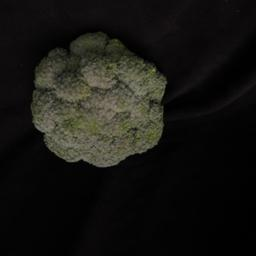
\includegraphics[width=\textwidth]{../results/q_samples/mis_rotten/OTHER_0_ROTTEN_3.jpg}
\captionsetup{labelformat=empty}
\caption{}
\end{subfigure}%
  \begin{subfigure}{.123\textwidth}
  \centering
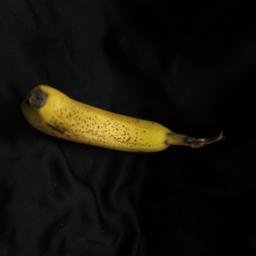
\includegraphics[width=\textwidth]{../results/q_samples/mis_rotten/RIPE_0_ROTTEN_2.jpg}
\captionsetup{labelformat=empty}
\caption{}
\end{subfigure}
 \vskip .1in
 %%%%%% non banana %%%%%%%%%
 \begin{subfigure}{.123\textwidth}
  \centering
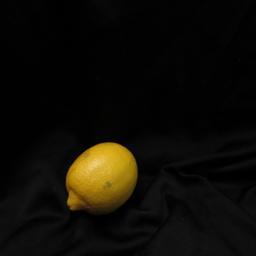
\includegraphics[width=\textwidth]{../results/q_samples/cor_other.jpg}
\captionsetup{labelformat=empty}
\caption{Other}
\end{subfigure}%
\qquad
 \begin{subfigure}{.123\textwidth}
  \centering
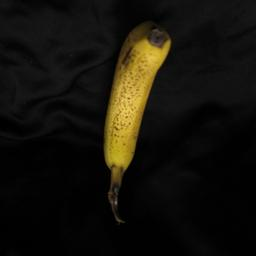
\includegraphics[width=\textwidth]{../results/q_samples/mis_other/RIPE_3_OTHER_2.jpg}
\captionsetup{labelformat=empty}
\caption{}
\end{subfigure}%
  \begin{subfigure}{.123\textwidth}
  \centering
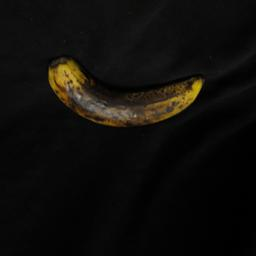
\includegraphics[width=\textwidth]{../results/q_samples/mis_other/ROTTEN_3_OTHER6.jpg}
\captionsetup{labelformat=empty}
\caption{}
\end{subfigure}%
  \begin{subfigure}{.123\textwidth}
  \centering
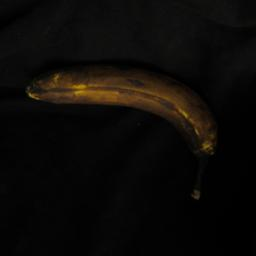
\includegraphics[width=\textwidth]{../results/q_samples/mis_other/ROTTEN_3_OTHER_3.jpg}
\captionsetup{labelformat=empty}
\caption{}
\end{subfigure}%
  \begin{subfigure}{.123\textwidth}
  \centering
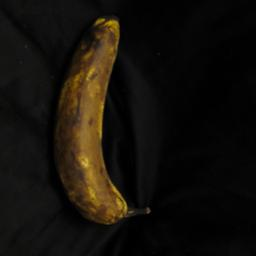
\includegraphics[width=\textwidth]{../results/q_samples/mis_other/ROTTEN_3_OTHER_6.jpg}
\captionsetup{labelformat=empty}
\caption{}
\end{subfigure}
\caption{Samples of correctly classified data from each class are presented in the first column. For each row, the remaining columns contain samples of incorrectly classified objects that have been given the same label as the object in the first column. }
\label{fig:correctVsIncorrect}
\end{figure}
\begin{itemize}
\item (RBF, FC6) improved the performance of~\citet{saad2009recognizing} in classifying banana ripeness with significantly larger data set.
\end{itemize}
\section{Discussion}
\label{sec:conclusion}
. This model could be very helpful in helping disabled people to detect the ripeness of bananas. In addition, it could become handy in industry for large scale sorting. 
\begin{itemize}
\item unbalanced set in banana vs objects. 
\item Successfully enhanced previous work by adding non-banana objects. 
\item Future: generalize ripeness detection to other fruits and vegetables. 
\item Industrial application: automatic large scale sorting. 
\item Mobile app for visually disabled: find the ripeness of fruits and vegetables via phone camera. 
\item Code and data set available at \href{bit.ly/BananaRipe}{bit.ly/BananaRipe}
\end{itemize}

\subsubsection*{Acknowledgments}
We thank our TA Zhiwei (Lucas) Deng and for his guidance on using Caffe as well as AlexNet. We also thank Dr. Mori for his insights on solving this problem. 
 
\renewcommand\refname{\vskip -.75cm}
\subsubsection*{References}

   \bibliography{report}		    
   \bibliographystyle{plainnat}
\end{document}
